%%%%%%%%%%%%%%%%%%%%%%%%%%
%                          %
% ----- INTRODUCTION ----- %
%                          %
%%%%%%%%%%%%%%%%%%%%%%%%%%

\section{Fonctionnalités}

	La deuxième itération de l'application vise à couvrir certaines autres fonctionnalités :
	\begin{itemize}
		\item Recherche d'informations dans la page "Cases" et "Patients"
		\item Page d'édition d'un "Case"
		\item Page d'édition d'un "Patient"
	\end{itemize}

\section{Conception}

	Le deuxième prototype de l'application comprend donc des nouveautés en termes de fonctionnalités. En effet, après avoir déployé et présenté le premier prototypes, des remarques de la part du client ont centré le développement sur les deux fonctionnalités suivantes les plus intéressantes; la recherche d'informations, et l'édition de données. La fonctionnalité principale est l'édition des données, et il fallait pouvoir éditer la plupart des données affichées : Aussi bien celles d'un cas que celles d'un patient.

	\section{Pages d'édition}
	
		Deux nouvelles pages sont donc consacrées à afficher et permettre la modification d'une part d'un cas, et d'autre part d'un patient. Ces pages sont accessibles en cliquant respectivement sur la ligne d'un, ou sur la ligne d'un patient dans la liste. Cette page affiche toutes les informations relatives au cas ou au patient concerné, mais chacune a une spécificité supplémentaire :

		\begin{itemize}
			\item La page "Case" affiche également les informations du Patient concerné, ainsi qu'un bouton "Edit" redirigeant l'utilisateur vers la page d'édition du Patient.
			\item Le page "Patient" affiche l'ensemble des cas qui concernent ce patient. Cliquer sur un cas dirige l'utilisateur vers la page d'édition de celui-ci.
		\end{itemize}

		La figure \ref{proto2_1} montre un prototype de la page de modification d'un cas.

		\begin{figure}[!h]
			\centering
			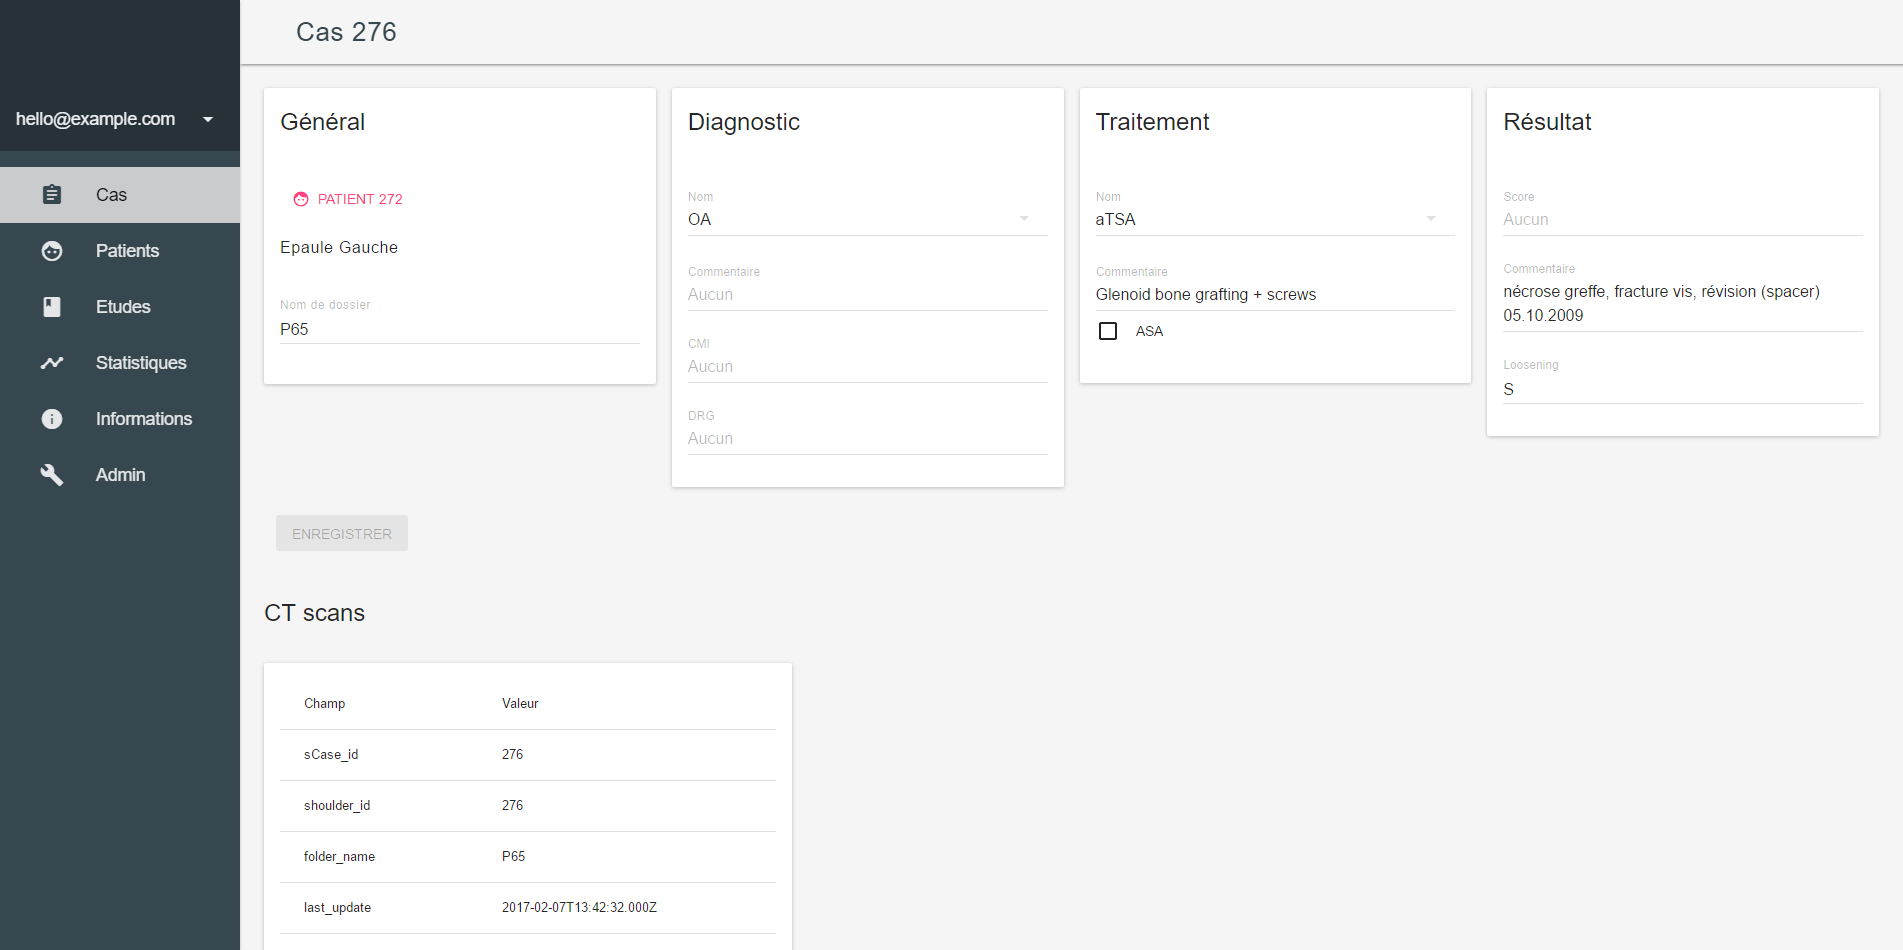
\includegraphics[width=1\textwidth]{images/realisation/proto2_1}
			\caption{Prototype de la page de modification d'un cas}
			\label{proto2_1}
		\end{figure}

	\section{Recherche}

		Une autre fonctionnalité a été modifiée : Le filtrage des données. Le système initial de filtres a été changé en un champ de recherche, qui est plus facile et plus rapide à utiliser. Ce filtre sera présent aussi bien sur la page Cases que sur la page Patients. Ecrire dans le champ recherche la chaîne de caractères entrée dans l'ensemble des champs des données affichées.
		La figure \ref{proto2_2} montre un prototype de la page de la liste des cas.

		\begin{figure}[!h]
			\centering
			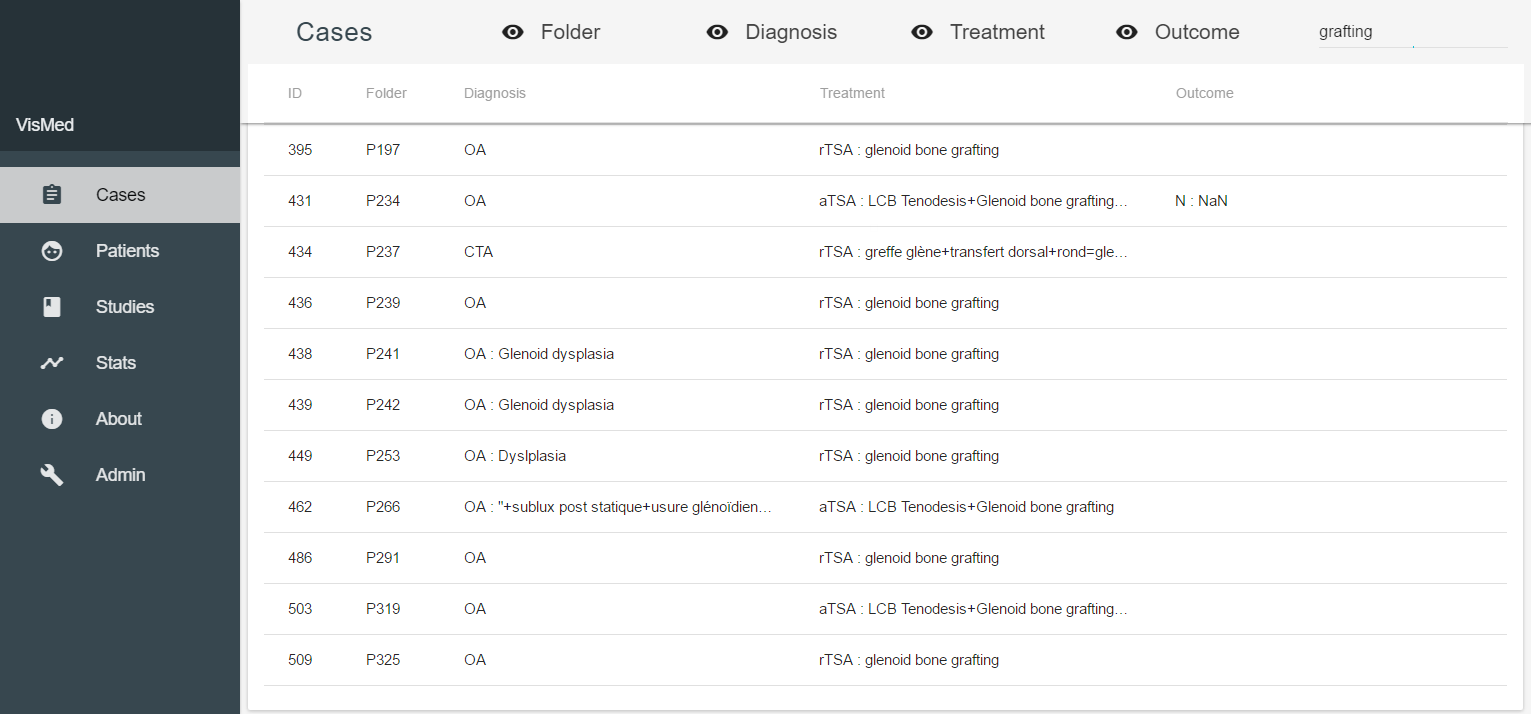
\includegraphics[width=1\textwidth]{images/realisation/proto2_2}
			\caption{Prototype de la liste des cas avec recherche de mot clé}
			\label{proto2_2}
		\end{figure}


\section{Implémentation}

	\subsection{Pages d'édition}

		L'implémentation des pages d'édition d'un cas et d'un patient s'est naturellement faite pas l'addition de deux nouveaux composants \texttt{Case} et \texttt{Patient}.

		\subsubsection{Case}

			Les données à afficher sur la page de Cas sont plus larges que les données affichées sur la liste des cas : En effet, il est nécessaire ici de montrer la liste des CT scans liés à un cas. Cet ajout a nécessité des modifications dans le backend : L'ajout d'un endpoint destiné à renvoyer non seulement toutes les informations d'un cas, mais également l'ensemble des informations des CT liés à ce cas.

			La méthode suivante a donc été ajoutée au serveur :
			\begin{description}
				\item[\texttt{GET /api/case/<id>}] Renvoie les informations du cas \texttt{<id>} ainsi que les CT qui sont liées
			\end{description}

			Celle-ci fait appel à une vue SQL implémentée sous le nom de \texttt{ct\_view}.

			De plus, la possibilité de modifier les données du cas a également nécessité tout d'abord l'ajout d'une méthode sur le serveur :

			\begin{description}
				\item[\texttt{POST /api/case/<id>}] Modifie les informations du cas \texttt{<id>}
			\end{description}

			Cette méthode fait appel à une procédure stockée SQL implémentée pour cette fonctionnalité. Nommée \texttt{updateCase}, elle prend en paramètre l'ensemble des données modifiables d'un cas. Si un paramètre est laissé vide (C'est le cas lorsqu'il n'est pas modifié par l'utilisateur dans l'interface), il est ignoré et n'est pas mis à jour. Ceci a été fait pour éviter le cas où plusieurs modifications concurrentes pourraient écraser des nouvelles données avec des données non mises à jour.

			Afin de repérer facilement quelles données vont être mises à jour, les champs modifiés dans l'interface sont également mis en surbrillance avec une couleur bleue. La figure montre un champ "Commentaire" modifié, qui se distingue des autres champs de sa catégorie.

			\begin{figure}[!h]
				\centering
				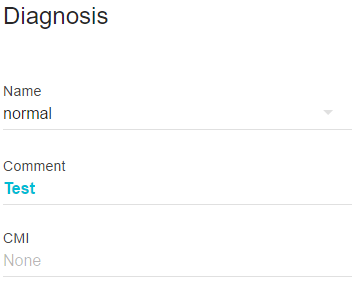
\includegraphics[width=0.4\textwidth]{images/realisation/proto2_3}
				\caption{Mise en évidence du champ modifié}
				\label{proto2_3}
			\end{figure}

		\subsubsection{Patient}

			L'ajout de la page de modification d'un Patient a demandé des efforts semblables à ceux de la page Case. On retrouve donc l'ajout de deux nouvelles méthodes à l'API, cette fois-ci pour un patient :

			\begin{description}
				\item[\texttt{GET /api/patient/<id>}] Renvoie les informations du patient \texttt{<id>} ainsi que des cas qui lui sont liées
				\item[\texttt{POST /api/patient/<id>}] Modifie les informations du patient \texttt{<id>}
			\end{description}

			Une des différences est que la méthode \texttt{GET /api/patient/<id>} renvoie également la liste des cas appartenant à un patient.

			De même, une procédure stockée SQL a également été implémentée pour permettre la modification facile des données d'un Patient, sous le nom de \texttt{updatePatient}.

	\subsection{Recherche}

		L'implémentation du champ de recherche ainsi que les boutons d'affichage des colonnes dans le \texttt{Header} a nécessité la création de composants spécialisées pour gérer ce type de Header, en dehors des Headers classiques. Les composants \texttt{CasesHeader} et \texttt{PatientsHeader} ont été crées, et affichent donc les contrôles nécessaires pour afficher ou cacher des colonnes, ainsi que gérer la recherche.

		Ces deux composants doivent communiquer avec les composants \texttt{Cases} et \texttt{Patients} de base. Il a donc été nécessaire de faire passer cette communication par le flux d'informations installé jusqu'ici.

		Lorsque l'utilisateur modifie l'affichage de colonnes ou la recherche appliqué, une action est donc crée et dispatchée sur le Store correspondant (soit CaseStore, soit PatientStore). La vue de la liste est ensuite mise à jour à partir des informations du store. Cependant, contrairement à précédemment, toute ces opérations se sont du côté client, et aucune communication avec le serveur n'est requise.

\section{Evaluation heuristique et adaptations}

	Au cours du développement de cette application, plusieurs évaluations formatives ont été réalisées. Chaque évaluation se focalise sur une ou plusieurs parties de l'application différentes, mais le but est généralement commun : On souhaite faire le point sur l'état actuel de l'utilisabilité de l'application en prenant un point de vue utilisateur, et en se posant des questions sur le design actuel de l'interface.

	Bien que fonctionnelle, ces vues n'étaient pas optimales sur le plan ergonomique. Une évaluation formative a montré plusieurs points à changer :
	\begin{itemize}
		\item La première information affichée sur la page Cas concerne le Patient : Cela est inadéquat
		\item Le bouton "Save" ne devrait concerner que la partie de la page effectivement modifiable
		\item Les champs d'input contiennent un label trop peu visible : Il est nécessaire d'améliorer leur visibilité
		\item Le champ de date est présent dans la base de données, mais pas sur la page : Il faut l'ajouter
	\end{itemize}

	Ces dernières remarques ont donc été prises en compte afin de réaliser la dernière version de l'interface de l'application.

\section{Résultat}

	L'application est fonctionnelle, et propose les éléments suivants :

	Les figures~\ref{cases1}, \ref{cases2} montrent respectivement la vue de la page de l'ensemble des Cas, ainsi que la vue de la page d'un Cas spécifique.

	\begin{figure}[!h]
		\centering
		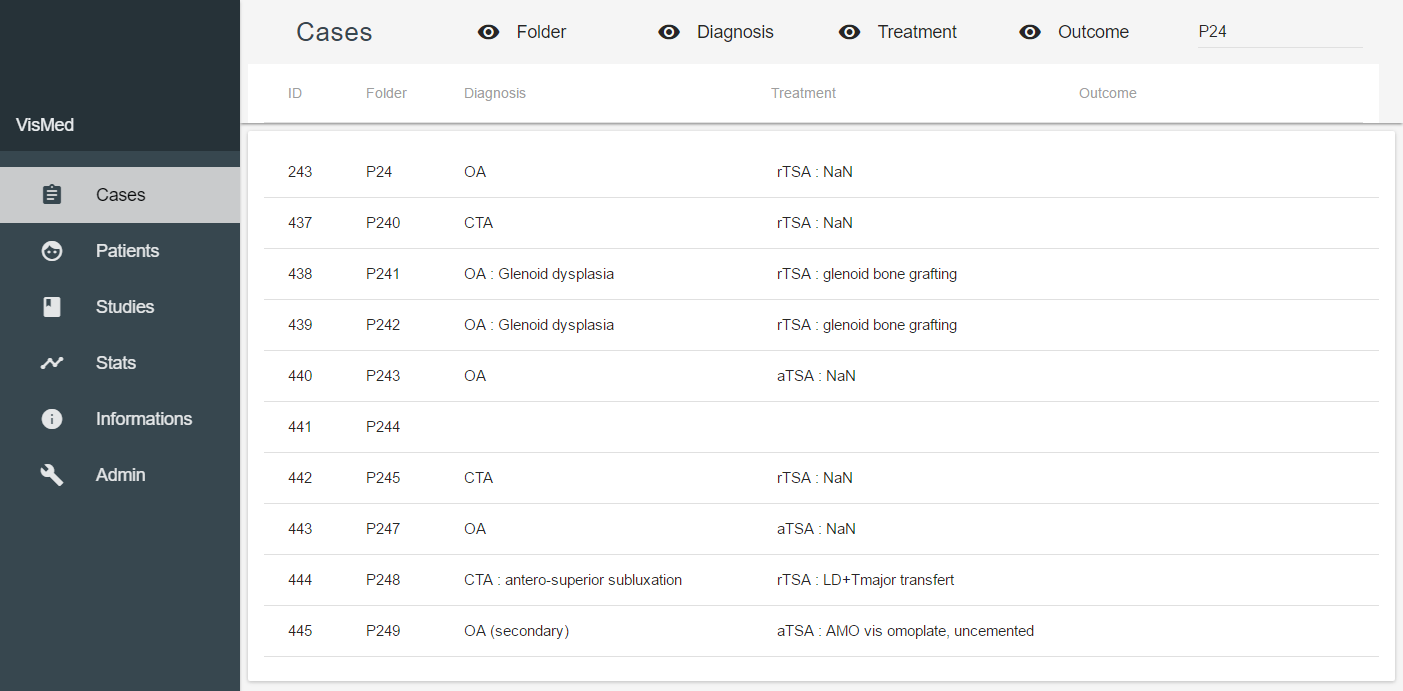
\includegraphics[width=1\textwidth]{images/realisation/cases1}
		\caption{Page "Cases" mise à jour, montrant la recherche de l'information 'P24'}
		\label{cases1}
	\end{figure}

	\begin{figure}[!h]
		\centering
		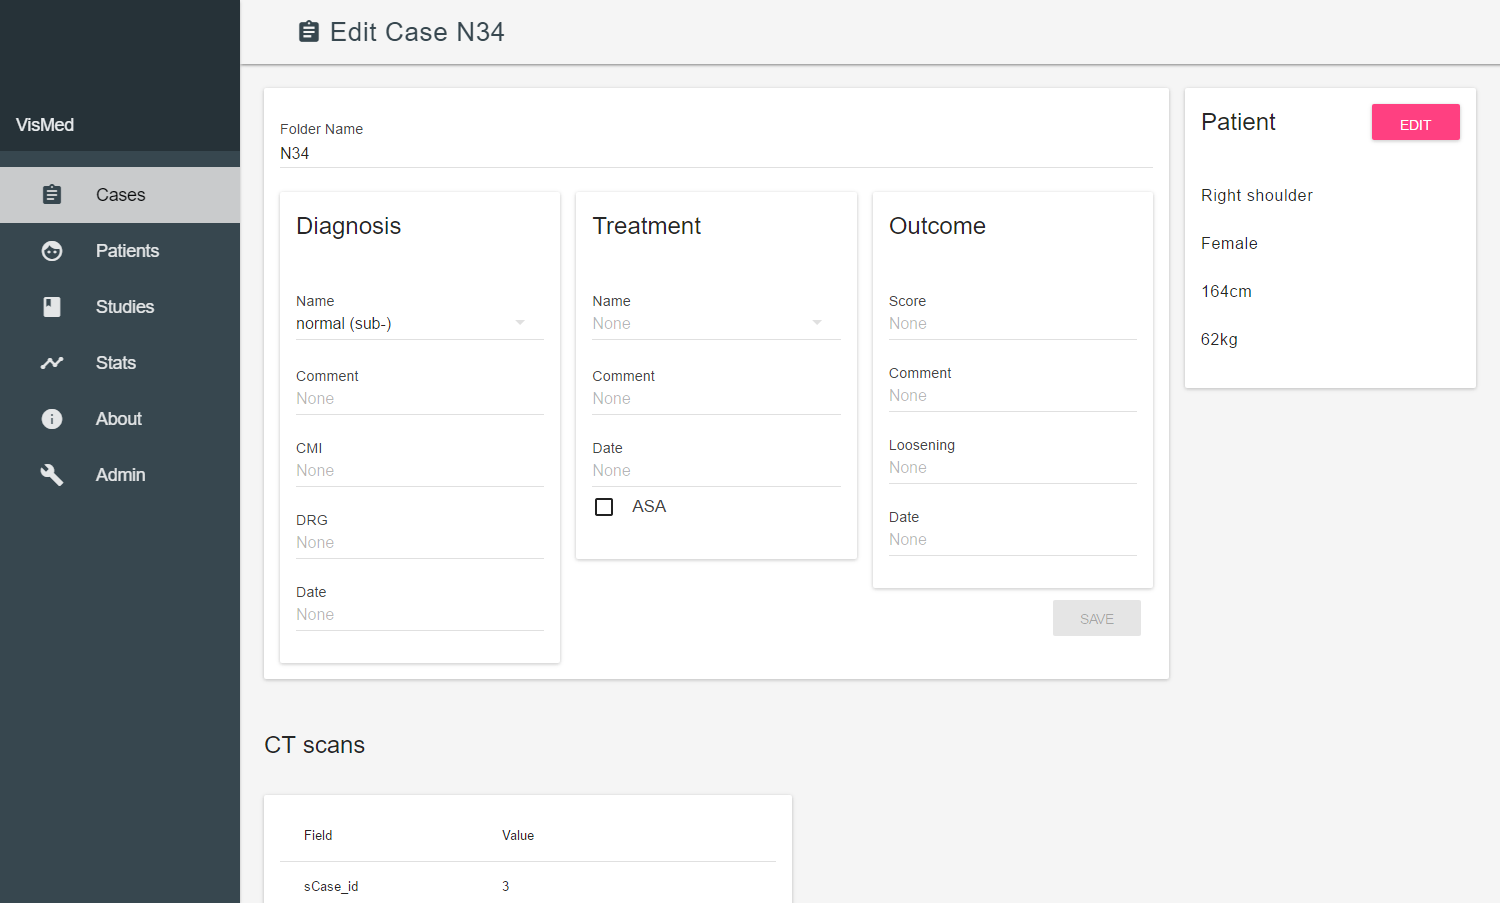
\includegraphics[width=1\textwidth]{images/realisation/cases2}
		\caption{Page finale d'édition d'un cas}
		\label{cases2}
	\end{figure}

	Les figures~\ref{patients1}, \ref{patients2} montrent respectivement la vue de la page de l'ensemble des Patients, ainsi que la vue de la page d'un Patient spécifique.

	\begin{figure}[!h]
		\centering
		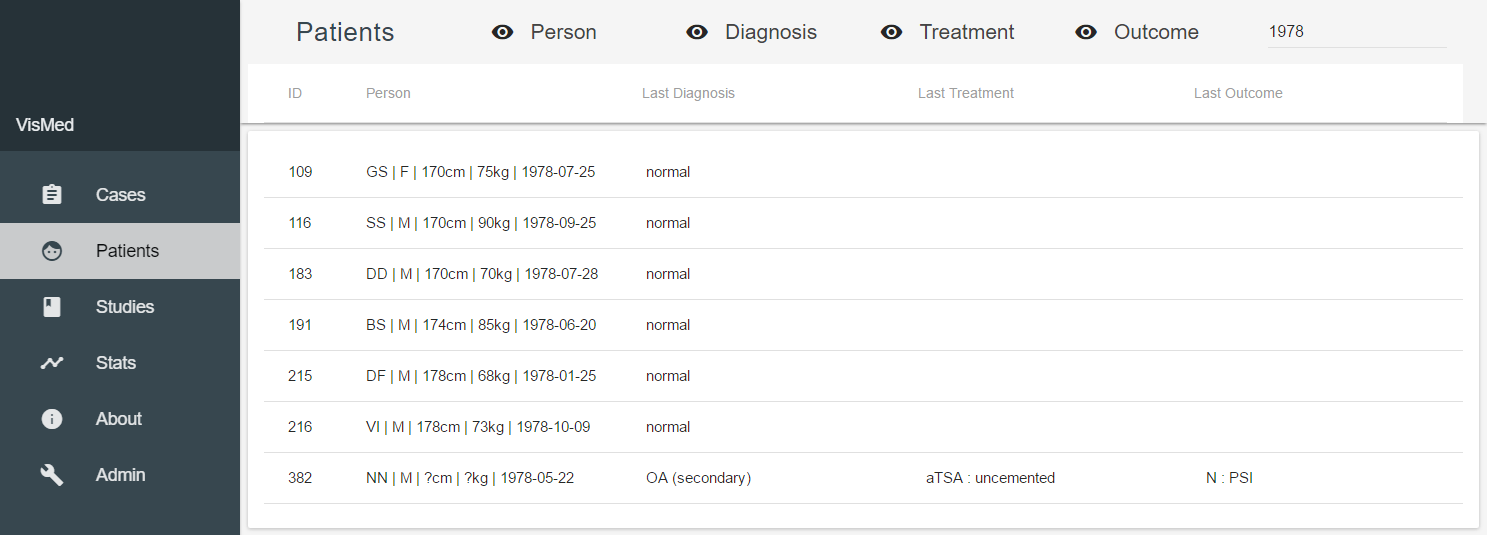
\includegraphics[width=1\textwidth]{images/realisation/patients1}
		\caption{Page "Patients" mise à jour, montrant la recherche de l'information '1980'}
		\label{patients1}
	\end{figure}

	\begin{figure}[!h]
		\centering
		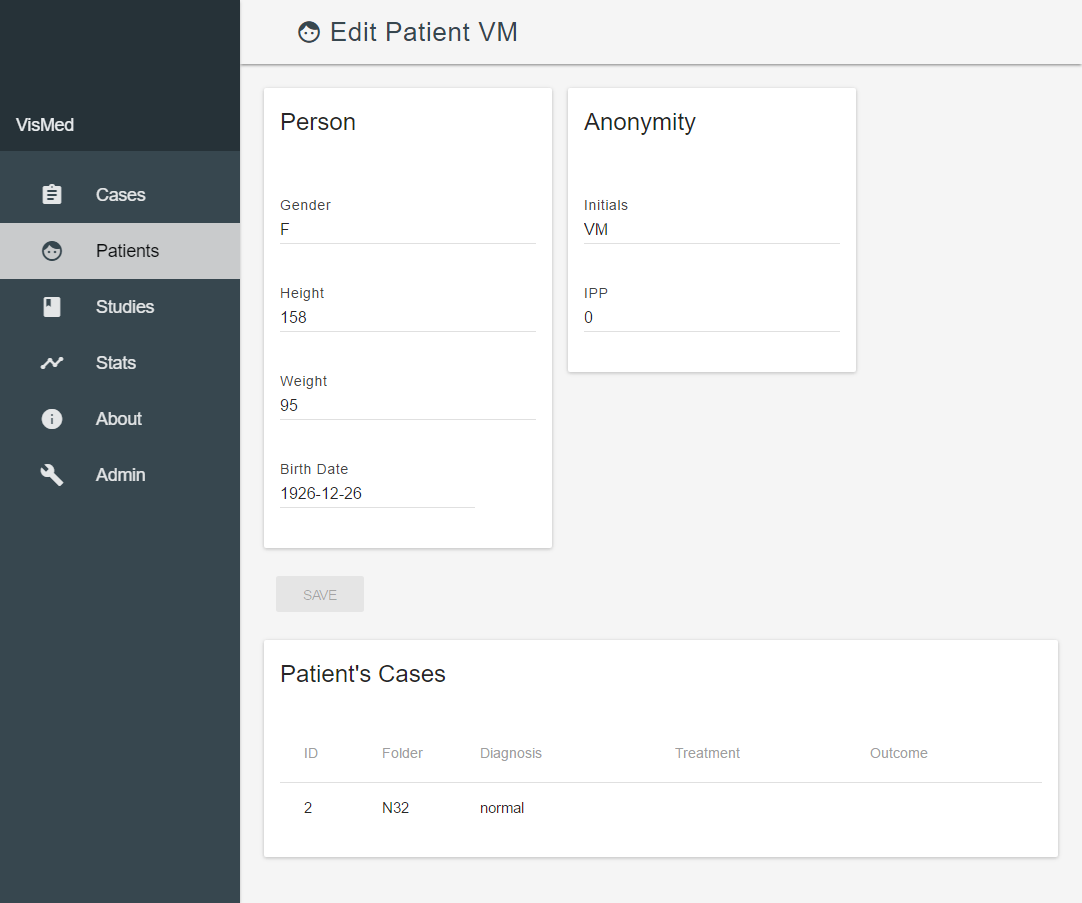
\includegraphics[width=1\textwidth]{images/realisation/patients2}
		\caption{Page finale d'édition d'un patient}
		\label{patients2}
	\end{figure}
